\chapter{Longlist verschillende AR / VR technologieën}
\label{ch:longlist}

Hierin worden de verschillende technologieën overlopen die kunnen gebruikt worden om deze use case te volbrengen.
Bij elke technologie zal er dan worden gezegd waarom deze voldoet of niet voldoet aan de eisen (TODO) van de use case.

\section{Head Mounted Virtual Reality}
Bij head mounted virtual reality wordt er gebruik gemaakt van een HDM (head-mounted-display) die de gebruiker op zijn hoofd zet. Deze headset zal dan een virtuele wereld tonen die volledig aangestuurd is door de applicatie zelf. Deze wereld zal dus geen rekening houden met de echte wereld, dit kan hierdoor wel voor problemen zorgen indien er geen sensor of camera aanwezig is die je tegenhoud om tegen muren te lopen.

HMD kan over 3DOF of 6DOF beschikken afhankelijk van de gebruikte headset. De 3DOF headsets zijn wel goedkoper dan de 6DOF en maken vaak gebruik van de smartphone om zo het beeld te kunnen tonen. 
% TODO CONTENT Iets over het beeld dat in 2 wordt gesplitst, op elke oog 1 beeld
% TODO ASK Is uitleg over hoe het beeld op de ogen wordt geprojecteerd en geinterpreteerd door de hersenen teveel of topic?
\subsection{Medische Klachten}
Sommige mensen kunnen bij het gebruik van een HDM ziek of misselijk worden. Dit wordt meestal veroorzaakt door een te klein of onnatuurlijk gezichtsveld (Field-Of-View, FoV) (INSERT CITE) of als de beweging in de applicatie wordt gedaan a.h.v. teleportatie. (INSERT CITE) Deze teleportatie beweging komt vooral voor bij 3DOF omdat hierbij er manieren zijn om de camerea te bewegen, namelijk teleportatie of via een joystick.

De tijd tussen de beweging in de echte wereld en de virtuele kan ook invloed hebben op virtual reality sickness indien deze te hoog is \autocite{Elbamby2018} en \autocite{DiZio2000}. 
% TODO TRANSLATE disconnection
Veel van deze problemen hebben te maken met de staat van de huidige hardware en hoe deze geen hogere FoV aan een hoge framerate kunnen ondersteunen. Een hoge en stabiele framerate is nodig indien om de gebruiker een aangename ervaring te geven. Een te lage framerate kan ervoor zorgen dat er (TRANSLATE) disconnection is tussen de beweging van de gebruiker en het gene dat effectief op het scherm gebeurt, dit kan voor frustratie zorgen.
\subsection{Sensoren}
% TODO ASK Extra uitleg over IMU of niet?
De soorten sensoren die gebruikt worden bij een HMD hangt af van de gewenste bewegingen. Als er alleen maar rotationale bewegingen nodig zijn kan een gyroscoop (bij smartphones) of een IMU, inertial measurement unit (bij standalone headsets) worden gebruikt om zo de yaw, pitch, roll te kunnen meten en hierop te kunnen reageren \autocite{LaValle2014}. Indien er ook positionale bewegingen nodig zijn moeten er infraroodsensoren in de kamer worden geplaatst om zo de headset te kunnen tracken. Deze sensoren zorgen er wel voor dat er meer voorbereiding nodig is alvorens de headset kan worden gebruikt.
\subsection{Realisme}
Omdat de headset het beeld op de beide ogen projecteert is er geen besef van de echte wereld en kan de virtuele wereld makkelijker als 'echt' worden ervaart. De headset zal ook gemonteerd zijn op het hoofd waardoor beide handen vrij zijn om acties uit te voeren. Hierdoor kunnen beide handen ook worden gezien in de virtuele wereld wat de ervaring nog meer realistischer maakt.
% TODO CONTENT Iets over latency => tijd tussen beweging hoofd en beweging in vr
\subsection{Interactiviteit}
De manier waarop de gebruiker zal interageren met de virtuele wereld zal afhangen van het aantal vrijheidsgraden bij 6DOF zal hij de mogelijkheid hebben om zelf te kunnen rondlopen in de wereld terwijl bij 3DOF dit a.h.v. een joystick of via teleportatie zal moeten. Er is ook altijd de mogelijkheid om controllers te gebruiken. Deze controllers zullen dan de mogelijkheid bieden om fysieke interacties te kunnen doen, bijvoorbeeld het oppakken van een virtueel object of door op één van de knoppen van de controller te duwen een actie uit te voeren.

\begin{figure}
    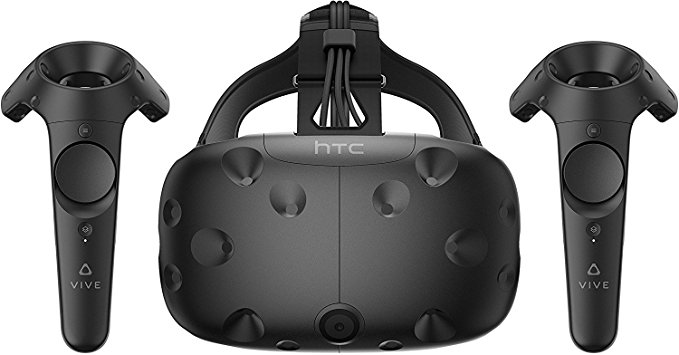
\includegraphics[width=\linewidth]{headset.jpg}
    \caption{HTC Vive headset en controllers}
    \label{fig:htcvive}
\end{figure}

\subsection{Bruikbaarheid}
De bruikbaarheid van HMD in musea is nogal laag. Het is niet echt praktisch om gebruikers met een HMD (Google Cardboard of Full HMD) te laten rondlopen omdat dit veel ruimte in het museum zou kosten om goed te implementeren. Indien er toch zou worden gekozen om dit te implementeren kan bij er ook een hoge financiele kost aanhangen. Afhankelijk of de gebruikers moeten langskomen voor de applicatie uit te proberen of niet kan het zijn dat het museum headsets moet aankopen en hiervoor een speciale ruimte moet inrichten.

Meeste mensen die naar een museum gaan willen juist rondlopen in het museum zelf rondlopen en niet in de virtuele versie hiervan. Het is daarom ook niet echt logisch om een HMD hiervoor te gebruiken. Natuurlijk als het museum wil gaan voor een ervaring zoals bij het Historium Brugge kan HMD wel op een goede manier worden gebruikt.

\section{Augmented Reality} \label{sec:augmentedreality}
Augmented reality kan het best worden omschreven als het plaatsen van virtuele objecten in de echte wereld zonder gebruik te maken van een headset. Omdat er geen headset wordt gebruikt zal de smartphone als vervanging dienen.
\subsection{Plane Detection}
Om virtuele objecten in de echte wereld te kunnen plaatsen moet de echte wereld eerst gemapped. Dit gebeurt a.h.v. computer vision om zo te weten waar een nieuwe plane begint en eindigt. Dit algoritme zal constant lopen om zo nieuwe planes te kunnen ontdekken \autocite{Xu2018}. 

Eens een plane ontdekt is kan deze worden gebruikt om nieuwe objecten op te plaatsen. De applicatie zal dan het object verbinden aan een ankerpunt (INSERT CITE). Door dit ankerpunt kan de locatie van het object worden onthouden zelfs als de gebruiker wat verder weg wandelend. Er zijn echter wel limieten aan dit anker, indien de gebruiker te ver weg gaat van het punt en nadien terug komt zal het virtuele object verplaatst zijn, dit begrip noemt drifting \autocite{You1999}. Indien er grote precisie nodig is voor de applicatie kan dit wel problemen zorgen.
% TODO IMAGE Point cloud / plane detection
% TODO CITE Object Anchor, alleen maar concrete implementaties gevonden ARCORE / ARKIT https://developers.google.com/ar/develop/developer-guides/anchors
% TODO CITE Drifting
\subsection{Image Recognition}
Een tweede manier om virtuele objecten in de wereld te plaatsen is met image recognition. Ook hierbij wordt gebruik gemaakt van computer vision zoals te zien op figuur \ref{fig:imagereg}.

Hierbij zal de image worden gebruikt als ankerpunt om de virtuele objecten op te plaatsen en te onthouden. Eens de image herkent is kunnen de objecten erop worden geplaatst. Wanneer de smartphone de afbeelding niet meer kan zien zal deze de positie van het object, na een tijdje, vergeten en zal tracking worden uitgezet. Vanaf de smartphone de afbeelding weer herkent kan het terug worden weergegeven.

Een alternatief van image recognition is object recognition. In plaats van een 2d afbeelding wordt er hier een 3d object gebruikt dat wordt herkent.

\begin{figure}
    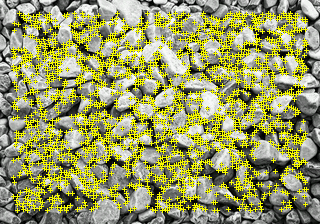
\includegraphics[width=\linewidth]{vuforiaImageReg.png}
    \caption{Aangeduide features op een afbeelding}
    \label{fig:imagereg}
\end{figure}

\subsection{Sensoren}
\subsection{Realisme}
\subsection{Interactiviteit}
\subsection{Bruikbaarheid}
\section{360 Degrees Videos}
\section{Mixed Reality} \label{sec:mixedreality}
Ook hierbij wordt er gebruik gemaakt van een HDM. Het grote verschil met virtual reality is dat er bij mixed reality ook rekening wordt gehouden met de echte wereld. Een mixed reality headset heeft namelijk de mogelijkheid om de echte wereld te mappen naar een virtuele wereld a.h.v. de camera die langs de voorkant gemonteerd is.

Een mixed reality headset is ook uitgerust met verschillende sensoren om de positie binnen in de wereld te volgen. Door de combinatie van de mapping en sensoren is het dus niet nodig om extra sensoren te plaatsen om room-scale VR te te gebruiken.
\subsection{Spatial Mapping}
Het algoritme dat gebruikt wordt voor de mapping is spatial mapping. Dit algoritme % TODO CONTENT Uitleg spatial mapping

% TODO CONTENT Alternative devices? AR glasses? Future of?